\newpage{}\section{Rappresentazione con CCS}

\subsection{Modellazione tramite CCS}\label{sec:ccs-model}

In prima battuta, è doveroso modellare il protocollo con il CCS(\emph{Calculus
of Communicating Systems}).

Vengono quindi individuati i seguenti agenti:

\begin{itemize}
\item \textbf{Memory}: cella di memoria in cui è possibile leggere o scrivere
  il numero di sequenza di un messaggio;
\item \textbf{Sender}: processo che legge continuamente il numero di sequenza
  corrente dalla memoria e trasmette un messaggio con numero di sequenza
  uguale all'esito di tali letture;
\item \textbf{Receiver}: processo che riceve i messaggi spediti da
  \textbf{Sender}, fornendo sempre conferme (\texttt{ACKX});
\item \textbf{BadReceiver}: variante del Receiver, non accetta sempre i
  messaggi in ingresso (fornisce sia \texttt{ACKX} che \texttt{NACKX});
\item \textbf{AckReceiver}: processo che rimane in ascolto di comunicazioni di
  corretta o errata ricezione da parte di un \textbf{Receiver} o un
  \textbf{BadReceiver}. \\
  Nel caso in cui un messaggio accompagnato da numero di sequenza X venga
  trasmesso correttamente, \textbf{AckReceiver} cambia il valore nella cella
  di memoria.
\end{itemize}

Gli agenti sopra menzionati usano i seguenti canali (per facilità di notazione
scritti usando il VP-CCS (\emph{Value Passing-CCS}));

\begin{itemize}
\item \textbf{read(x)}: canale utilizzato per leggere lo stato della cella di
  memoria. \\
  L'argomento \texttt{x} è lo stato salvato in \textbf{Memory};
\item \textbf{write(x)}: canale utilizzato per aggiornare lo stato della cella
  di memoria. \\
  L'argomento \texttt{x} è lo stato che si vuole scrivere in \textbf{Memory};
\item \textbf{msg(x)}: canale utilizzato per mandare un messaggio da
  \textbf{Sender} a \textbf{Receiver}. \\
  Ha come argomento il numero di sequenza \texttt{x} associato al messaggio
  spedito;
\item \textbf{ack(x)}: canale utilizzato per confermare la corretta ricezione
  del messaggio avente numero di sequenza \texttt{x};
\item \textbf{nack(x)}: canale utilizzato per notificare l'errata ricezione
  del messaggio avente numero di sequenza \texttt{x};
\item \textbf{ok(x)}: canale utilizzato per notificare la corretta trasmissione
  del messaggio avente numero di sequenza \texttt{x};
\end{itemize}

Viene quindi esposto in CCS come gli agenti comunicano tra di loro affinchè i
requisiti esposti in sezione \ref{sec:intro} siano soddisfatti: \\

$ $

$ > Memory_0 := \overline{read}_0.Memory_0 + write_1.Memory_1 $

$ > Memory_1 := \overline{read}_1.Memory_1 + write_0.Memory_0 $

$ $

$ > Sender := read_0.(\overline{msg}_0.Sender + read_1.Sender) +
              read_1.(\overline{msg}_1.Sender + read_0.Sender) $

$ $

$ > Receiver_0 := msg_0.\overline{ack}_0.Receiver_1 $

$ > Receiver_1 := msg_1.\overline{ack}_1.Receiver_0 $

$ $

$ > BadReceiver_0 := msg_0.(\overline{ack}_0.BadReceiver_1 +
                            \overline{nack}_0.BadReceiver_0) $

$ > BadReceiver_1 := msg_1.(\overline{ack}_1.BadReceiver_0 +
                            \overline{nack}_1.BadReceiver_1) $

$ $

$ > AckReceiver_0 := ack_0.AckReceiver_{M0} +
                     nack_0.AckReceiver_0 + ack_1.AckReceiver_0) $

$ > AckReceiver_{M0} := \overline{write}_1.ok_0.AckReceiver_1 $

$ > AckReceiver_1 := ack_1.AckReceiver_{M1} +
                     nack_1.AckReceiver_1 + ack_0.AckReceiver_1) $

$ > AckReceiver_{M1} := \overline{write}_0.ok_1.AckReceiver_0 $

$ $

$ > Sys_{Reliable} =  (Sender | Receiver_0 | AckReceiver_0 | Memory_0) $
  \textbackslash{} $ \{msg_0,msg_1,read_0,read_1,write_0,write_1,
                       ack_0,ack_1,nack_0,nack_1\} $

$ $

$ > Sys_{Unreliable} =  (Sender | BadReceiver_0 | AckReceiver_0 | Memory_0) $
  \textbackslash{} $ \{msg_0,msg_1,read_0,read_1,write_0,write_1,
                       ack_0,ack_1,nack_0,nack_1\} $

\begin{figure}[H]
  \centering
  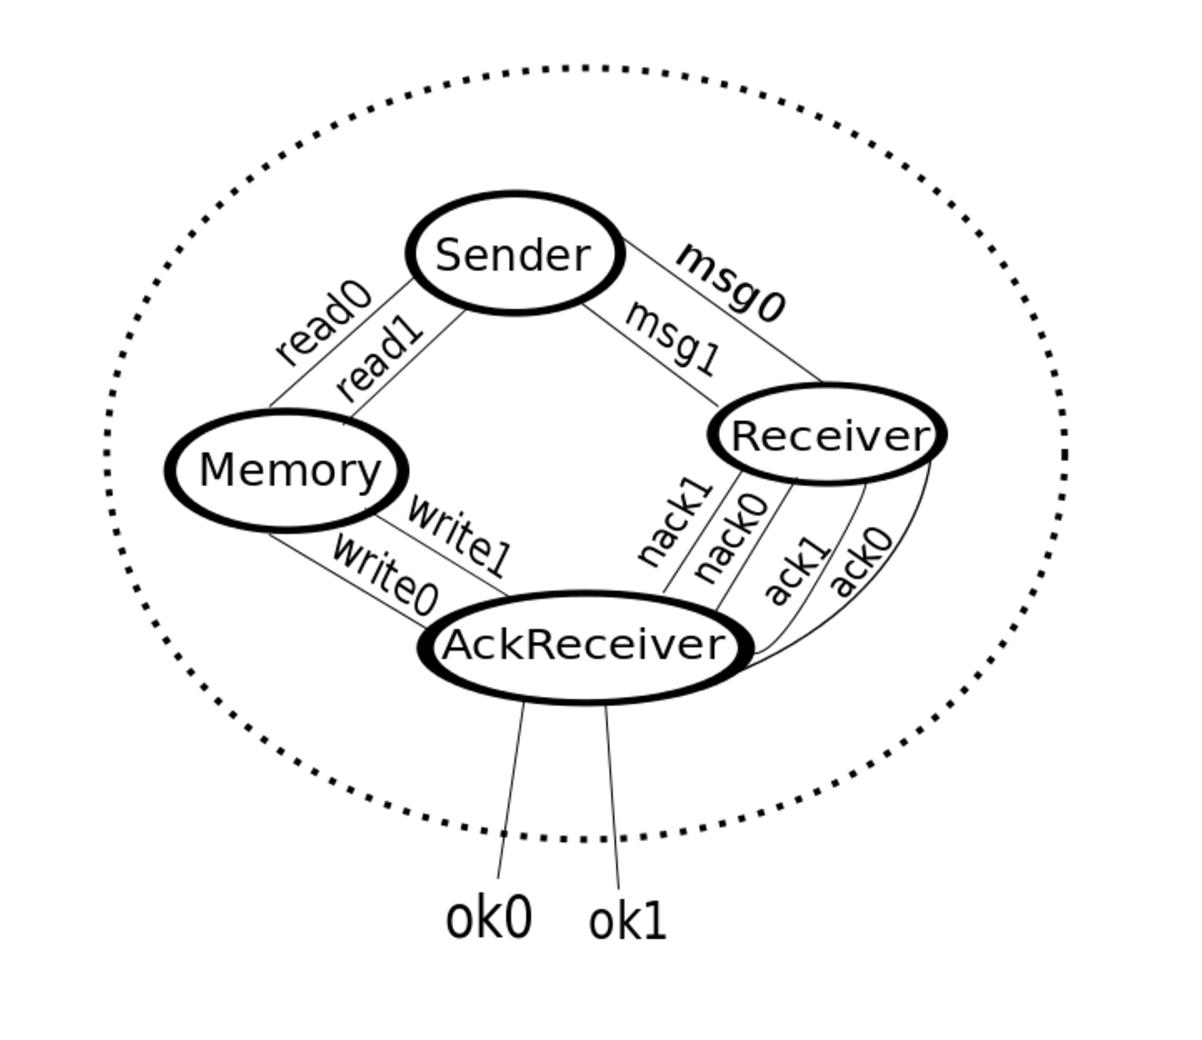
\includegraphics[width=.5\columnwidth]{images/ccs.eps}
  \caption{Rappresentazione di ABP tramite CCS}
  \label{fig:ccs-abp}
\end{figure}

\subsection{pseuCo}

Il sistema è stato provato anche su \url{pSeuco.com} (script
\ref{sec:pseuco-script}). 

Sebbene il grafico risultante è piuttosto confusionario, sembra che la
rappresentazione del sistema in CCS soddisfi le proprietà attese.

Ad esempio, non vi è nessun cerchio blu nel \emph{LTS}, ovvero non vi è alcun
deadlock.

Nella parte superiore del grafico vi sono tutte le notifiche da parte di
\texttt{$AckReceiver_1$} di corretta ricezione, mentre nella parte inferiore
quelle di \texttt{$AckReceiver_0$}:

\begin{figure}[H]
  \centering
  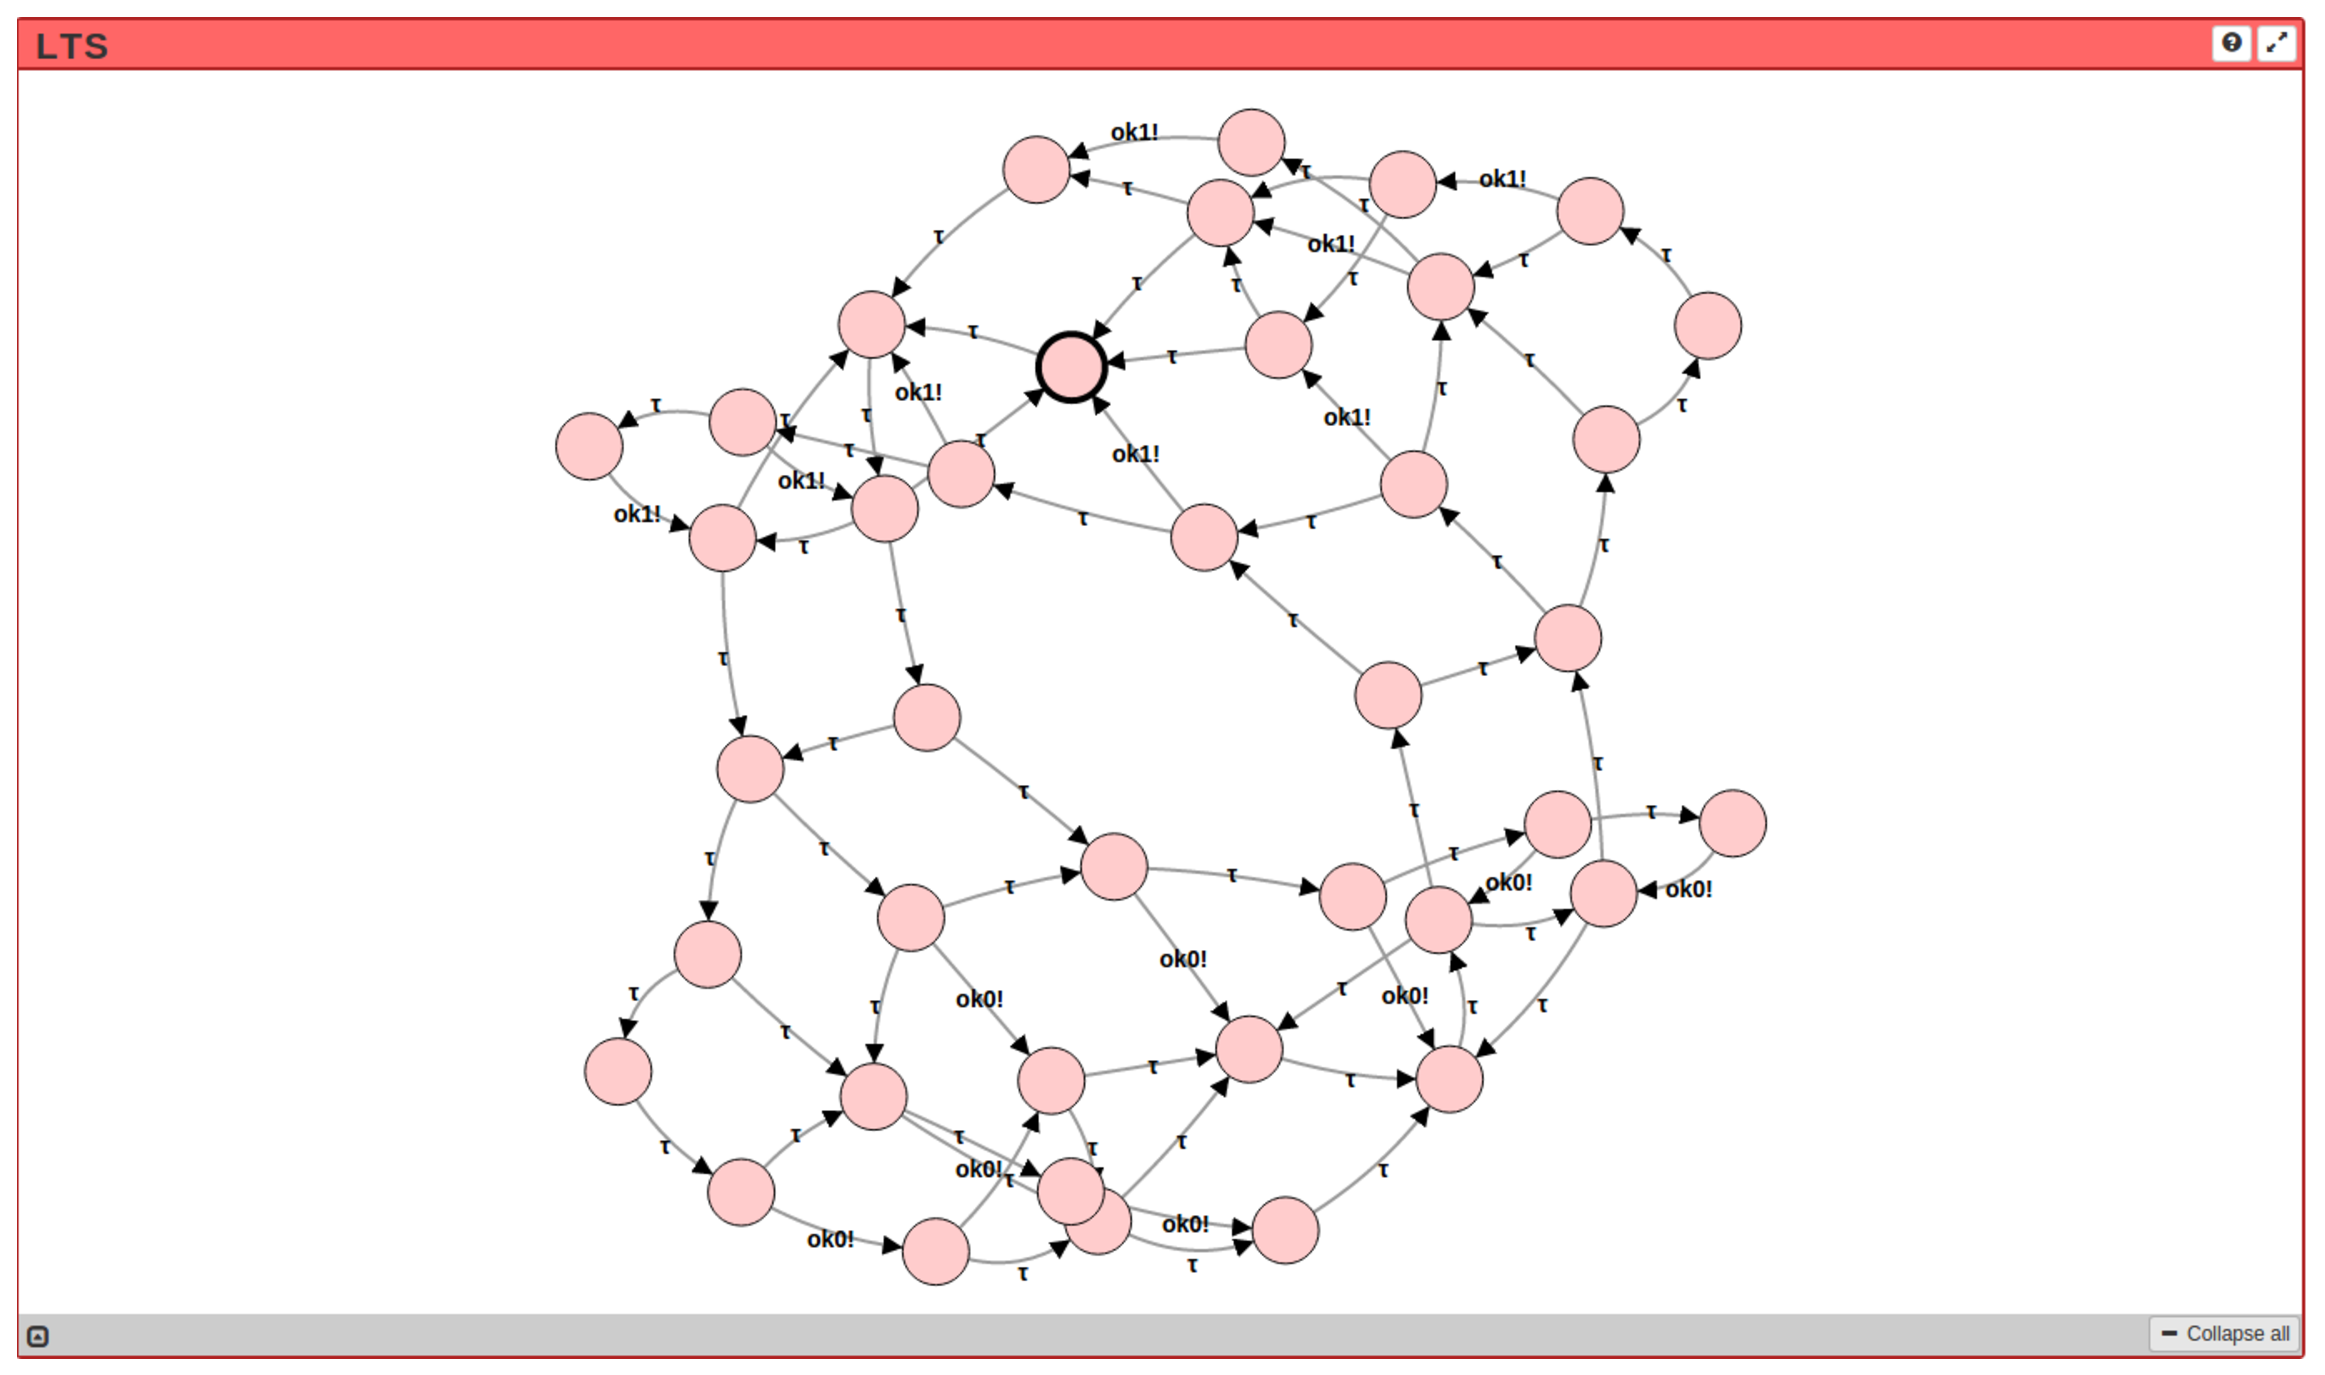
\includegraphics[width=.8\columnwidth]{images/pseuco.eps}
  \caption{\emph{LTS} disegnando da pseuCo}
  \label{fig:ccs-abp}
\end{figure}
